\documentclass[a4paper,12pt, oneside]{book}

%\usepackage{fullpage}
\usepackage[italian]{babel}
\usepackage[utf8]{inputenc}
\usepackage{amssymb}
\usepackage{amsthm}
\usepackage{graphics}
\usepackage{amsfonts}
\usepackage{listings}
\usepackage{amsmath}
\usepackage{amstext}
\usepackage{engrec}
\usepackage{rotating}
\usepackage[safe,extra]{tipa}
\usepackage{showkeys}
\usepackage{multirow}
\usepackage{hyperref}
\usepackage{microtype}
\usepackage{enumerate}
\usepackage{braket}
\usepackage{marginnote}
\usepackage{pgfplots}
\usepackage{cancel}
\usepackage{polynom}
\usepackage{booktabs}
\usepackage{enumitem}
\usepackage{framed}
\usepackage{pdfpages}
\usepackage{pgfplots}
\usepackage[cache=false]{minted}
\usepackage{fancyhdr}
\pagestyle{fancy}
\fancyhead[LE,RO]{\slshape \rightmark}
\fancyhead[LO,RE]{\slshape \leftmark}
\fancyfoot[C]{\thepage}



\title{BrainJobs}
\author{UniShare\\\\Davide Cozzi\\\href{https://t.me/dlcgold}{@dlcgold}\\\\Gabriele De Rosa\\\href{https://t.me/derogab}{@derogab}}}
\date{}

\pgfplotsset{compat=1.13}
\begin{document}
\maketitle

\definecolor{shadecolor}{gray}{0.80}

\newtheorem{teorema}{Teorema}
\newtheorem{definizione}{Definizione}
\newtheorem{esempio}{Esempio}
\newtheorem{corollario}{Corollario}
\newtheorem{lemma}{Lemma}
\newtheorem{osservazione}{Osservazione}
\newtheorem{nota}{Nota}
\newtheorem{esercizio}{Esercizio}
\tableofcontents
\renewcommand{\chaptermark}[1]{%
	\markboth{\chaptername
		\ \thechapter.\ #1}{}}
\renewcommand{\sectionmark}[1]{\markright{\thesection.\ #1}}

\chapter{Introduzione}
BrainJobs è un (ipotetico) servizio cloud di tipo Software-as-a-Service (SaaS) che offre ai
suoi utenti la possibilità di “allenare” modelli di apprendimento automatico, di valutarne le
prestazioni ed (eventualmente) riutilizzarli per effettuare simulazioni.
Il sistema permette agli utenti di effettuare richieste di allenamento o simulazione caricando i
dati insieme al modello o utilizzandone uno già precedentemente allenato e salvato nel
proprio archivio. In base al linguaggio o al framework utilizzato per il codice del modello,
BrainJobs lancia la computazione in un particolare ambiente di esecuzione che verrà
istanziato “on-the-fly” in un’altra piattaforma cloud di tipo Serverless basata su containers
(es: Apache OpenWhisk, Knative, ...).
Gli utenti possono sottomettere più richieste consecutive. Esse verranno gestite in parallelo
in un sistema a coda. Ogni richiesta di un utente corrisponde ad un task di lavoro (job).
Gli utenti possono controllare lo stato delle loro richieste dalla dashboard di BrainJobs, ed
una volta terminate, visualizzarne i risultati. Successivamente, il sistema permette di scartare
o salvare il modello per utilizzi futuri.
L’architettura del servizio BrainJobs è suddivisa in tanti servizi e componenti, ognuno con un
compito ben specifico. Al vostro team, è richiesta la creazione di due componenti:
\begin{enumerate}
\item un componente di frontend implementato utilizzando HTML, CSS e JavaScript che
  utilizza il paradigma AJAX per inviare/ricevere dati
\item un componente di backend che espone una HTTP API REST
\end{enumerate}
Il frontend deve permettere ad un utente di creare una nuova richiesta di allenamento,
visualizzare la lista delle sue richieste e visualizzare le informazioni di dettaglio di ogni
richiesta.
Il backend deve essere in grado di salvare una nuova richiesta, fornire la lista delle richieste
di un utente e restituire informazioni di dettaglio di ogni richiesta.
Una volta che il backend ha salvato una nuova richiesta, altri servizi di BrainJobs si
occuperanno di lanciare la computazione, aggiornare lo stato del job ed aggiungere i
risultati.\\
\begin{figure}[h!]
  \centering
  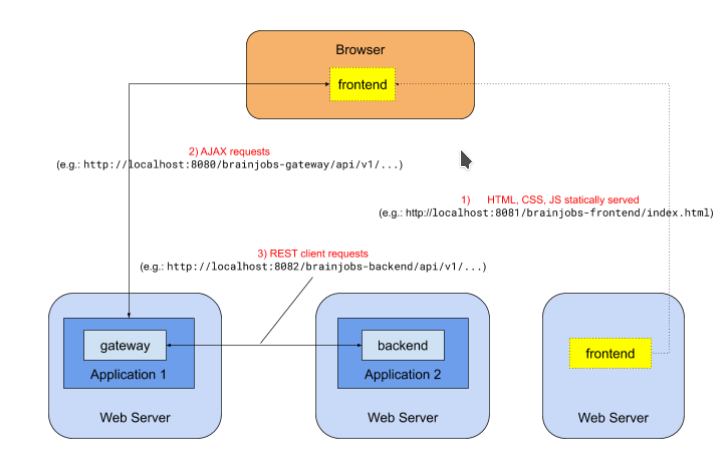
\includegraphics[scale = 0.7]{img/struttura.png}
  \caption{struttura finale del progetto}
\end{figure}
\chapter{FrontEnd}
Iniziamo parlando del frontend. Per quanto riguarda l'aspetto estetico è stato usato un tema di Bootstrap
per poter rappresentare più semplicemente componenti come il menù presente nella parte alta
della pagina, contenente le informazioni del progetto, e la navbar con il bottone per richiamare il menù. Entrambi componenti sono nel tag \textit{header}.

\begin{figure}[h!]
  \centering
  
\includegraphics[scale = 0.385]{img/navbar.png}
  \caption{navbar}
\end{figure}
\begin{figure}[h!]
  \centering
  
\includegraphics[scale = 0.385]{img/menu.png}
  \caption{menù a scomparsa}
\end{figure}

\textbf{navbar}:
\begin{shaded}
\begin{minted}{html}
<div class="navbar navbar-dark bg-dark shadow-sm">
 <div class="container d-flex justify-content-between">
  <a href="#" class="navbar-brand d-flex align-items-center">
   <strong><i class="fas fa-brain"></i> BrainJobs</strong>
   </a>
   
  <button class="navbar-toggler" type="button"
    data-toggle="collapse"
    data-target="#navbarHeader" aria-controls="navbarHeader"
    aria-expanded="false" aria-label="Toggle navigation">
   <span class="navbar-toggler-icon"></span>
  </button>
 </div>
</div>
\end{minted}
\end{shaded}
\textbf{Menù:}
\begin{shaded}
\begin{minted}{html}
<div class="collapse bg-dark" id="navbarHeader">
 <div class="container">
  <div class="row">
   <div class="col-sm-8 col-md-7 py-4">
    <h4 class="text-white">Informazioni</h4>
    <p class="text-muted">
     Progetto del corso di Sistemi Distribuiti dell'anno
      accademico 2018/19 all'università degli studi di
       Milano-Bicocca.
    </p>
   </div>
   <div class="col-sm-4 offset-md-1 py-4">
    <h4 class="text-white">Crediti</h4>
     <ul class="list-unstyled">
      <li><a class="text-white"
       href="https://www.github.com/dlcgold">
        Davide Cozzi</a></li>
      <li><a class="text-white"
       href="https://www.github.com/derogab">
        Gabriele De Rosa</a></li>
     </ul>
    </div>
   </div>
  </div>
</div>
\end{minted}
\end{shaded}
Si passa poi alla sezione con il titolo della pagina, con l'icona presa da quella
messe a disposizione sul sito \url{https://fontawesome.com/icons/}:
\begin{figure}[h!]
  \centering
  
\includegraphics[scale = 0.8]{img/titolo.png}
  \caption{titolo della pagina}
\end{figure}
\begin{shaded}
\begin{minted}{html}
<section class="jumbotron text-center">
 <div class="container">
  <h1 class="jumbotron-heading"><i class="fas fa-brain"></i>
   BrainJobs</h1>
 </div>
</section>
\end{minted}
\end{shaded}
Analizziamo ora una delle parti principali della pagina: \textbf{il form di inserimento dati}. Qui si è fatto uso della classe \textit{form-group} per impostare i
vari campi del form, con titolo e \textit{form-control} per l'inserimento, e della
classe \textit{custom-select} per quei campi con selezione obbligatoria,
dove quindi è stato aggiunto un selettore:
\begin{figure}[H]
  \centering
  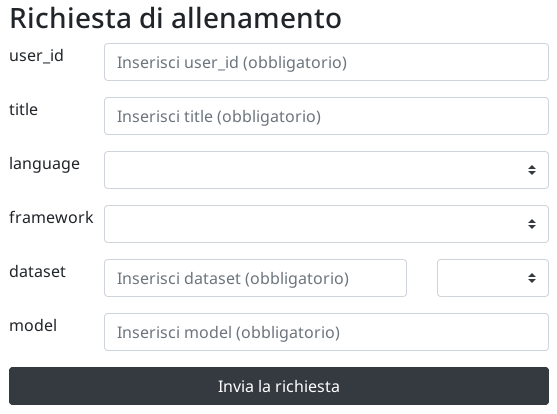
\includegraphics[scale = 0.7]{img/form.png}
  \caption{form per l'inserimento della richiesta}
\end{figure}
\begin{figure}[H]
  \centering
  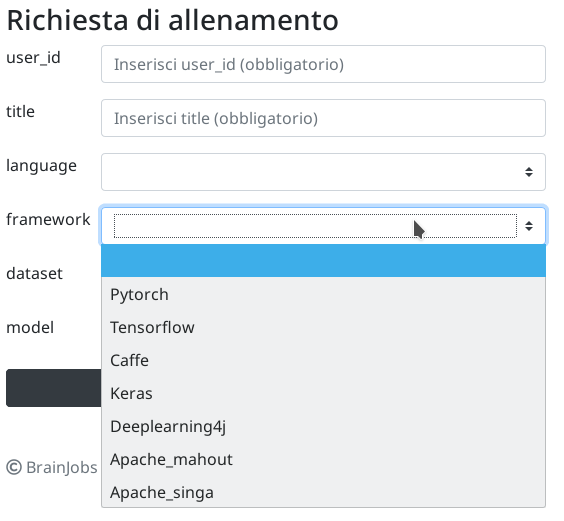
\includegraphics[scale = 0.7]{img/selettore.png}
  \caption{esempio di selettore}
\end{figure}

Vediamo quindi, per esempio, la parte nell'\textit{index.html} dedicata all'inseriemnto di \textit{title}, ovvero un inserimento manuale senza selettore:
\begin{shaded}
\begin{minted}{html}
<div class="row">
 <div class="col-md-2 col-sm-12">
  <label for="title">title</label>
 </div>
 <div class="col-md-10 col-sm-12">
  <input type="text" class="form-control" id="title"
   placeholder="Inserisci title (obbligatorio)">
 </div>
</div>
\end{minted}
\end{shaded}
Dove notiamo come le classi \textit{col-md-n} e \textit{col-sm-n} permettono di rendere \textit{responsive} gli elementi (la stringa e il box di inserimento).
\newpage
Passiamo ora a vedere l'esempio di un inserimento mediante selettore, prendendo come esempio
l'inserimento del framework:
\begin{shaded}
\begin{minted}{html}
<div class="form-group">
 <div class="row">
  <div class="col-md-2 col-sm-12">
   <label for="framework">framework</label>
  </div>
  <div class="col-md-10 col-sm-12">
   <select class="custom-select" class="form-control"
     id="framework">
    <option selected></option>
    <option value="pytorch">Pytorch</option>
    <option value="tensorflow">Tensorflow</option>
    <option value="caffe">Caffe</option>
    <option value="keras">Keras</option>
    <option value="deeplearning4j">Deeplearning4j</option>
    <option value="apache_mahout">Apache_mahout</option>
    <option value="apache_singa">Apache_singa</option>
   </select>
  </div>
 </div>
</div>
\end{minted}
\end{shaded}
Analizziamo ora la seconda parte fondamentale della pagina, dove l'utente può
inserire uno \textit{user\_id} o un \textit{job\_id} per effettuare una query nel database
delle richieste:
\begin{figure}[H]
  \centering
  
\includegraphics[scale = 0.8]{img/query.png}
  \caption{campi per l'inserimento di query}
\end{figure}
\newpage
Nell'\textit{index.html} si ha quindi:
\begin{shaded}
\begin{minted}{html}
<h3>Dettagli</h3>

<h6>Richieste di uno user</h6>
 <div class="row">
  <div class="col-md-6">
   <input type="text" class="form-control"
     id="user_id_search"
      placeholder="Inserisci lo user_id">
  </div>
  <div class="col-md-6">
   <button id="get-all-requests"
     class="btn btn-dark btn-block">
      Visualizza le richieste di user</button>
  </div>
 </div>

 <h6 style="margin-top: 10px;">Richiesta singola</h6>
 <div class="row">
  <div class="col-md-6">
   <input type="text" class="form-control"
     id="job_id" placeholder="Inserisci job_id">
  </div>
  <div class="col-md-6">
   <button id="get-single-request"
    class="btn btn-dark btn-block">
     Visualizza la richiesta</button>
  </div>
 </div>
\end{minted}
\end{shaded}
infine i risulati della query verranno visualizzati mediante:
\begin{shaded}
\begin{minted}{html}
<div id="results"></div>
\end{minted}
\end{shaded}
\newpage
Infine una parola per tutta quella parte del file dedicata al permettere l'uso di \textit{bootstrap}, \textit{jquery}
e del \textit{custom.js} mediante il quale, con l'uso di \textbf{ajax}, sono state fatte le \textit{POST} e le \textit{GET}:
\begin{shaded}
\begin{minted}{html}
<!-- nell'HEAD -->
    
<!-- Bootstrap core CSS -->
<link href="css/bootstrap.min.css" rel="stylesheet">

<!-- FA -->
<link href="css/fa.css" rel="stylesheet">

<!-- Custom styles for this template -->
<link href="css/custom.css" rel="stylesheet">

...


<!-- alla fine del file -->

<!-- jQuery -->
<script src="js/jquery.min.js"></script>
<script>window.jQuery ||
 document.write('<script src="js/jquery.min.js">
  <\/script>')</script>
    
<!-- Bootstrap bundle JS -->
<script src="js/bootstrap.bundle.min.js"></script>

<!-- Custom javascript script w/ ajax requests-->
<script src="js/custom.js"></script>
\end{minted}
\end{shaded}
\newpage
Abbiamo visto il file \textit{HTML} ma questo non basta in quanto serve il \textit{custom.js} per interagire, mediante jquery e ajax, con il backend. Si ha quindi la seguente struttura per il \textbf{frontend}:
\begin{shaded}
\begin{minted}{shell}
.
├── css:
│   ├── bootstrap.css
│   ├── bootstrap.css.map
│   ├── bootstrap-grid.css
│   ├── bootstrap-grid.css.map
│   ├── bootstrap-grid.min.css
│   ├── bootstrap-grid.min.css.map
│   ├── bootstrap.min.css
│   ├── bootstrap.min.css.map
│   ├── bootstrap-reboot.css
│   ├── bootstrap-reboot.css.map
│   ├── bootstrap-reboot.min.css
│   ├── bootstrap-reboot.min.css.map
│   ├── custom.css
│   ├── fa.css
│   └── fa.min.css
├── index.html
├── js:
│   ├── bootstrap.bundle.js
│   ├── bootstrap.bundle.js.map
│   ├── bootstrap.bundle.min.js
│   ├── bootstrap.bundle.min.js.map
│   ├── bootstrap.js
│   ├── bootstrap.js.map
│   ├── bootstrap.min.js
│   ├── bootstrap.min.js.map
│   ├── custom.js
│   ├── fa.js
│   ├── fa.min.js
│   ├── jquery.js
│   └── jquery.min.js
└── webfonts:
    ├── fa-brands-400.eot
    ├── fa-brands-400.svg
    ├── fa-brands-400.ttf
    ├── fa-brands-400.woff
    ├── fa-brands-400.woff2
    ├── fa-regular-400.eot
    ├── fa-regular-400.svg
    ├── fa-regular-400.ttf
    ├── fa-regular-400.woff
    ├── fa-regular-400.woff2
    ├── fa-solid-900.eot
    ├── fa-solid-900.svg
    ├── fa-solid-900.ttf
    ├── fa-solid-900.woff
    └── fa-solid-900.woff2
\end{minted}
\end{shaded}
con tutti i file per la parte di CSS, tutto il necessario per jquery e bootstrap, i fonts etc...\\
Ci concentriamo ovviamente sul \textit{custom.js} che abbiamo scritto per interfacciare frontend e backend.\\
Aprendo il file notiamo innanzitutto una definizione di costante:
\begin{shaded}
\begin{minted}{js}
const API = "http://localhost:8080/brainjobs-gateway/api/v1/";
\end{minted}
\end{shaded}
questa rappresenta parte del path per i vari endpoint presenti nel gateway.\\
Proseguendo oltre incontriamo la prima funzione di \textbf{jQuery} che controlla che quanto
è contenuto al suo interno venga eseguito unicamente una volta che il \textbf{DOM}
sia pronto per l'esecuzione di codice javascript:
\begin{shaded}
\begin{minted}{js}
\$(document).ready(function(){
 ...
});
\end{minted}
\end{shaded}
Passiamo ora ad analizzare le tre operazioni base che vengono effettuate.\\
Nell'\textit{index.html} il bottone associato all'invio di una richiesta
era stato identificato con l'id \textit{send-form} possiamo quindi sfruttare il metodo
\textit{.click()} di jquery per triggerare una funzione \textit{function(e)
} con una sequenza di istruzioni ogni volta che viene clickato il bottone.
Vediamo quindi queste istruzioni nel caso dell'invio del form.\\
Innanzitutto abbiamo un'struzione per prevenire l'azione di default di un evento (\textit{e}), evitando quindi il refresh della pagina:
\begin{shaded}
\begin{minted}{js}
 e.preventDefault();
\end{minted}
\end{shaded}
Definiamo poi una variabile per ogni campo del form sfruttando il metodo di jquery
\textit{.val()} che resituisce il valore di un id:
\begin{shaded}
\begin{minted}{js}
 var user_id = \$("#user_id").val();
 var title = \$("#title").val()
 var language = \$("#language").val();
 var framework = \$("#framework").val();
 var dataset = \$("#dataset").val();
 var dataset_datatype = \$("#dataset_datatype").val();
 var model = \$("#model").val();
\end{minted}
\end{shaded}
La traccia impone l'obbligo di avere tutti i campi compilati tranne quello riguardante
il framework, che è opzionale. Una if con la condizione che basti l'assenza
di uno dei campi viene usata per restituire, mediante l'id \textit{send-form-result}
e il metodo \textit{.html}, un alert, con un bottone dedicato alla sua chiusura:
\begin{shaded}
\begin{minted}{js}
if (!user_id || !title || !language ||
     !dataset || !dataset_datatype || !model ) { 
\$('#send-form-result').html(
   '<div class="alert alert-warning alert-dismissible fade show"
     role="alert">'
     +'<strong>Warning!</strong> Compilare i campi obbligatori.'
     +'<button type="button" class="close"
        data-dismiss="alert" aria-label="Close">'
     +'<span aria-hidden="true">&times;</span>'
     +'</button>'
     +'</div>');
 }
\end{minted}
\end{shaded}
\begin{figure}[H]
  \centering
  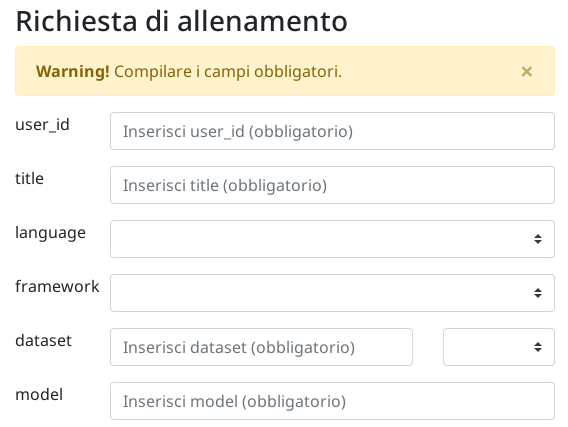
\includegraphics[scale = 0.7]{img/err-form.png}
  \caption{alert nel caso di form incompleto}
\end{figure}
Nel caso invece di form inserito correttamente si può procedere, mediante l'else, con la richiesta \textbf{ajax}.\\
\begin{shaded}
In informatica AJAX, acronimo di Asynchronous JavaScript and XML, è una tecnica di sviluppo software per la realizzazione di applicazioni web interattive (Rich Internet Application). Lo sviluppo di applicazioni HTML con AJAX si basa su uno scambio di dati in background fra web browser e server, che consente l'aggiornamento dinamico di una pagina web senza esplicito ricaricamento da parte dell'utente.

AJAX è asincrono nel senso che i dati extra sono richiesti al server e caricati in background senza interferire con il comportamento della pagina esistente. Normalmente le funzioni richiamate sono scritte con il linguaggio JavaScript. Tuttavia, e a dispetto del nome, l'uso di JavaScript e di XML non è obbligatorio, come non è detto che le richieste di caricamento debbano essere necessariamente asincrone. 
\end{shaded}
Si usa quindi il metodo \textit{\$.ajax()}, a cui viene specificato, mediante il campo
\textit{type}, il tipo di richiesta, mediante il campo \textit{url}, l'endpoint,
mediante il campo \textit{dataType}, il tipo di dato che ci si aspetta dal server,
mediante il campo \textit{data}, i dati che devono essere mandati al server, mediante il campo \textit{success}, la funzione che deve essere eseguita
se la richeista avviene con successo, e, mediante il campo \textit{error}, la funzione da eseguire in caso di errore.\\
Nel nostro caso queste ultime due funzioni sono due alert che avvisano se la richiesta è stata effettuata on successo o meno:
\begin{figure}[H]
\centering
\begin{minipage}{.5\textwidth}
  \centering
  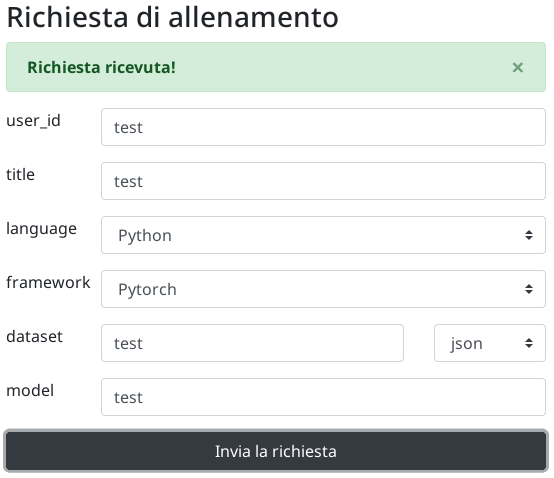
\includegraphics[scale = 0.42]{img/good-form.png}
  \caption{alert in caso di successo}
\end{minipage}%
\begin{minipage}{.5\textwidth}
  \centering
  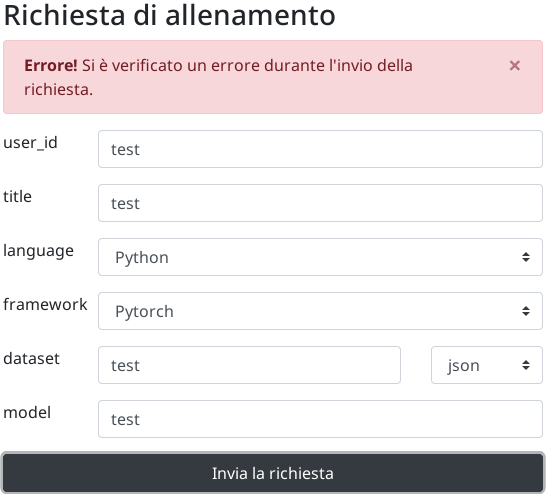
\includegraphics[scale = 0.4]{img/bad-form.png}
  \caption{alert in caso di errore}
\end{minipage}
\end{figure}
Passiamo ora alla prima delle due query, quella nel quale si inserisce uno \textit{user\_id} per ottenere tutte le richieste da lui effettuate. Come prima procediamo al click sul bottone, stavolta con l'id \textit{get-all-requests}, e salviamo in una variabile lo user_id:

\begin{shaded}
\begin{minted}{js}
\$(document).ready(function() {
  var user_id = \$("#user_id_search").val();
  e.preventDefault();
  ...
});
\end{minted}
\end{shaded}
\newpage
Anche qui con un if controlliamo che sia stato effettivamente inserito uno user\_id prima di effettuare la query premendo il bottone e in caso contrario si provvede a stampare un alert dedicato:

\begin{shaded}
\begin{minted}{js}
 if( !user_id ) {
  \$('#results').html('<div class="alert alert-warning
    alert-dismissible fade show" role="alert">'
   +'<strong>Warning!</strong> Compila il campo user_id.'
   +'<button type="button" class="close" data-dismiss="alert
    " aria-label="Close">'
   +'<span aria-hidden="true">&times;</span>'
   +'</button>'
   +'</div>');
 }
\end{minted}
\end{shaded}
\begin{figure}[H]
  \centering
  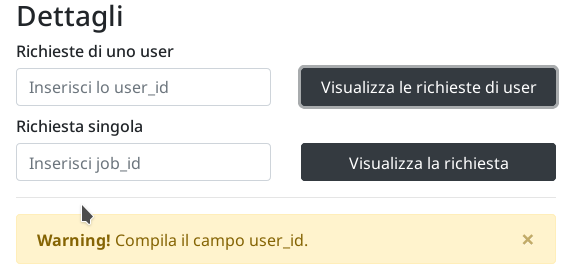
\includegraphics[scale = 0.7]{img/bad-user.png}
  \caption{alert nel caso di assenza di inserimento dello user}
\end{figure}
Altrimenti, mediante l'else, effettuiamo una richiesta di tipo \textit{GET} mediante ajax.
Si hanno due casi di successo, il primo se la richiesta avviene correttamente ma non
si hanno richieste per quello user\_id, la seconda se si ha invece almeno una richiesta.
Nel primo caso si controlla che l'array contenente le informazioni abbia lunghezza 0,
in tal caso si stampa un alert.
\begin{figure}[H]
  \centering
  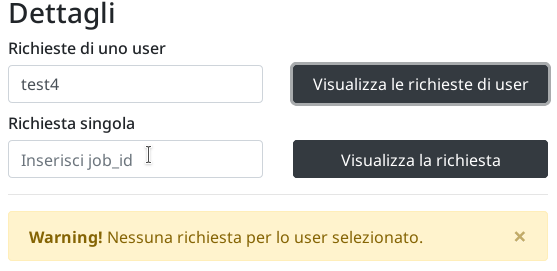
\includegraphics[scale = 0.7]{img/no-user.png}
  \caption{alert nel caso di assenza di richieste}
\end{figure}
Nel secondo caso,
mediante il metodo \textit{.each(function)} che permette di iterare su un oggetto
jquery permettendo di eseguire una \textit{function} per ogni elemento, stampo i
vari campi di ogni richiesta che mi viene resitutita dal server salvando progressivamente il tutto in una stringa \textit{result} che verrà associata all'id omonimo nell'\textit{index.html}. \\
\begin{figure}[H]
  \centering
  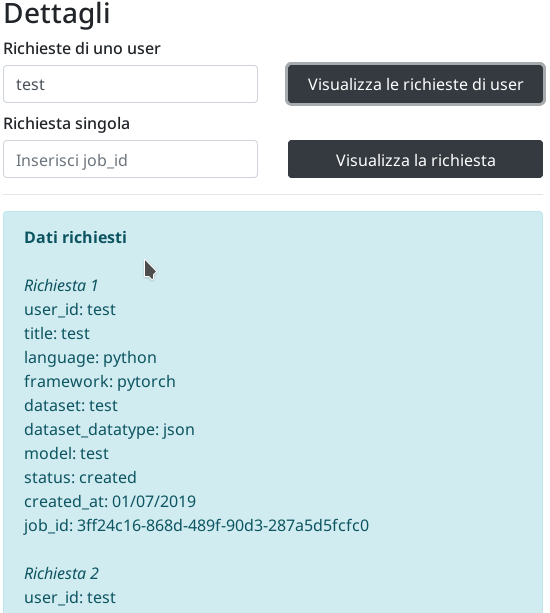
\includegraphics[scale = 0.65]{img/good-user.png}
  \caption{risultati in caso di presenza di richieste}
\end{figure}
\newpage
In caso di \textit{error} invece si avrà il solito alert:
\begin{figure}[H]
  \centering
  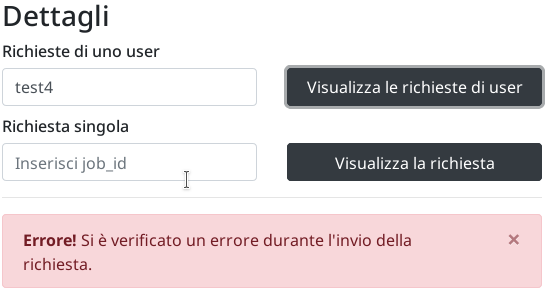
\includegraphics[scale = 0.7]{img/bad-user-query.png}
  \caption{alert in caso di errore nella richiesta ajax}
\end{figure}
\end{document}